\documentclass[12pt]{article}
\usepackage[polish]{babel}
\usepackage[utf8]{inputenc}
\usepackage{hyperref}
\usepackage{graphicx}
\usepackage{enumitem}
\usepackage{url}
\usepackage{listings}
\usepackage{booktabs}
\usepackage{multirow}
\usepackage{float}
\usepackage{titlesec}
\usepackage{xcolor}
\graphicspath{ {../images/} }

% Configure hyperlinks
\hypersetup{
    colorlinks=true,
    linkcolor=blue,
    filecolor=magenta,
    urlcolor=blue,
    pdftitle={System e-Toll - Dokumentacja},
    pdfauthor={},
    pdfsubject={Wymagania funkcjonalne i niefunkcjonalne systemu e-Toll},
    pdfkeywords={e-Toll, wymagania, architektura, system}
}

\title{System e-Toll}
\author{Dokumentacja systemu do zbierania danych na temat ruchu pojazdów\\po polskich drogach i naliczania należności za przejazdy}
\date{\today}

\begin{document}

\maketitle

\begin{center}
\url{https://github.com/Artur-Romaniuk/ais}\\
\url{https://www.overleaf.com/project/67e843e5c78b52b01a88211a}
\end{center}

\section*{Wstęp}
System e-Toll do zbierania danych na temat ruchu pojazdów po polskich drogach i naliczania należności za przejazdy.

\section*{Zakres dokumentu}
Rezultatem projektu powinien być dokument PDF, zawierający następujące elementy:

\begin{enumerate}
    \item Wymagania funkcjonalne.
    \begin{itemize}
        \item pogrupowana lista wymagań
        \item zidentyfikować jeden kluczowy proces biznesowy i szczegółowo ten proces zdefiniować. Definicja procesu to po prostu:
        \begin{itemize}
            \item cel procesu
            \item stan początkowy
            \item stan końcowy
            \item kroki procesu, z uwzględnieniem sytuacji wyjątkowych.
        \end{itemize}
    \end{itemize}
    
    \item Wymagania niefunkcjonalne.
    \begin{itemize}
        \item geograficzna skala działania
        \item liczba obsługiwanych klientów
        \item liczba obsługiwanych zdarzeń biznesowych w określonym czasie (na godzinę/dziennie/miesięcznie etc.)
        \item wymagania wydajnościowe
        \item wymagania niezawodnościowe
        \item wymagania bezpieczeństwa
        \item ...
    \end{itemize}
    
    \item Projekt systemu w postaci modelu C4 (\url{https://c4model.com/})
    \begin{itemize}
        \item wystarczą 3 pierwsze poziomy: context, containers, components, nie wymagam poziomu code
        \item diagram dynamiczny (dynamic diagram) realizujący opisany w wymaganiach proces biznesowy
        \item diagram wdrożenia (deployment diagram)
    \end{itemize}
    
    \item Dyskusja zastosowanych wzorców i/lub taktyk architektonicznych - w celu wyboru odpowiednich rozwiązań należy się odwołać do wymagań funkcjonalnych i niefunkcjonalnych.
    
    \item Decyzje architektoniczne w postaci modelu MAD 2.0
\end{enumerate}

\section{Wymagania funkcjonalne}

\subsection{Kluczowy proces biznesowy: Naliczanie i pobieranie opłat za przejazd}

\subsubsection{Cel procesu}
\begin{enumerate}
    \item Wykrywanie pojazdów na płatnych odcinkach dróg
    \item Naliczanie należności zgodnie z taryfami
    \item Pobieranie opłat od użytkowników
\end{enumerate}

\subsubsection{Stan początkowy}
Pojazd niezarejestrowany w systemie jako znajdujący się na płatnym odcinku drogi, z kontem użytkownika posiadającym określony stan środków (prepaid) lub limitem kredytowym (postpaid).

\subsubsection{Stan końcowy}
Prawidłowo naliczona i pobrana opłata za przejazd, zaksięgowana w systemie finansowym, z wygenerowanym potwierdzeniem dla użytkownika oraz aktualizacją stanu konta.

\subsubsection{Kroki procesu}
\begin{enumerate}
    \item Identyfikacja pojazdu wjeżdżającego na płatny odcinek (poprzez urządzenie OBU, aplikację mobilną lub kamery ANPR) [Dla redundancji, im więcej systemów tym większa szansa na identyfikację]
    \item Zebranie danych o pojeździe (kategoria, klasa emisji spalin, masa)
    \item Rozpoczęcie śledzenia przejazdu i rejestracja czasu wjazdu
    \item Monitorowanie trasy przejazdu przez punkty kontrolne
    \item Identyfikacja zjazdu z płatnego odcinka
    \item Obliczenie należności na podstawie przebytej trasy i charakterystyki pojazdu
    \item Weryfikacja dostępności środków na koncie użytkownika
    \item Pobranie opłaty z konta użytkownika
    \item Wygenerowanie potwierdzenia transakcji
    \item Aktualizacja salda konta użytkownika
\end{enumerate}

\paragraph{Obsługa sytuacji wyjątkowych:}
\begin{itemize}
    \item Jeśli identyfikacja pojazdu nie jest możliwa: uruchomienie procedury rejestracji incydentu z dokumentacją wizualną (zdjęcia niezidentyfikowanego pojazdu)
    
    \item W przypadku niewystarczających środków na koncie:
    \begin{enumerate}
        \item Zablokowanie konta do momentu zapłacenia
        \item W przypadku braku zapłaty w określonym czasie, uruchomienie procedury windykacyjnej
    \end{enumerate}
    
    \item Przy awarii urządzenia OBU: automatyczne przełączenie na identyfikację przez system kamer ANPR
    
    \item W razie przerwy w komunikacji: lokalne buforowanie danych i synchronizacja po przywróceniu łączności
    
    \item Jeśli zidentyfikowano omijanie bramek:
    \begin{enumerate}
        \item Poinformowanie użytkownika
        \item Uruchomienie procedury kontrolnej
        \item Naliczenie kary
    \end{enumerate}
\end{itemize}

\subsection{Lista wymagań funkcjonalnych}

\begin{enumerate}
    \item \textbf{System rejestracji użytkowników} - System musi umożliwiać rejestrację nowych użytkowników z weryfikacją tożsamości, zbieraniem danych o pojazdach (w tym masa, klasa emisji, kategoria) oraz wyborem metody płatności (prepaid lub postpaid).

    \item \textbf{Moduł geolokalizacji pojazdów} - System musi określać pozycję pojazdów z dokładnością do 10 metrów, wykorzystując dane GPS z urządzeń OBU lub aplikacji mobilnej, aktualizowane nie rzadziej niż co 30 sekund podczas przejazdu.

    \item \textbf{System rozpoznawania tablic rejestracyjnych (ANPR)} - System musi identyfikować pojazdy poprzez kamery ANPR z dokładnością co najmniej 98\% w różnych warunkach pogodowych i oświetleniowych, jako dopełnienie jeśli wszystkie systemy działają poprawnie lub alternatywa dla urządzeń OBU w razie awarii.

    \item \textbf{Elastyczny system taryfowy} - System musi obsługiwać zróżnicowane taryfy opłat w zależności od: typu pojazdu, masy całkowitej, klasy emisji spalin, pory dnia, dnia tygodnia oraz stopnia zatłoczenia drogi.

    \item \textbf{Moduł rozliczeń i płatności} - System musi obsługiwać różne metody płatności (karty płatnicze, przelewy, płatności mobilne, blik) z możliwością automatycznego doładowania konta prepaid oraz wystawiania faktur elektronicznych zgodnych z przepisami prawa.

    \item \textbf{System powiadomień dla użytkowników} - System musi wysyłać automatyczne powiadomienia do użytkowników (aplikacja, mail + sms) o: niskim stanie konta, zbliżającym się terminie płatności, dokonanych transakcjach oraz zmianach w taryfach i regulaminie.

    \item \textbf{Moduł raportowania i analityki} - System musi generować raporty dotyczące natężenia ruchu, generowanych przychodów, incydentów oraz efektywności egzekwowania opłat, z możliwością eksportu danych w formatach CSV i PDF.

    \item \textbf{System wykrywania naruszeń} - System musi identyfikować próby obejścia opłat (np. manipulacja urządzeniem OBU, podawanie fałszywych danych o pojeździe) i automatycznie uruchamiać procedury weryfikacyjne.

    \item \textbf{Portal samoobsługowy dla użytkowników} - System musi udostępniać portal internetowy oraz aplikację mobilną umożliwiającą użytkownikom zarządzanie kontem, przeglądanie historii przejazdów i opłat, generowanie raportów oraz aktualizację danych pojazdu.

    \item \textbf{System korekty opłat} - System musi umożliwiać ręczną korektę naliczonej opłaty przez operatora w przypadku zgłoszenia błędu przez użytkownika. Zakładając, że system źle naliczył opłatę np. Użytkownik został obciążony za trasę, której nie przejechał lub przypisano niewłaściwą kategorię pojazdu. Użytkownik zgłasza błąd do obsługi systemu. W takim przypadku operator musi mieć możliwość ręcznej korekty naliczonej opłaty np. Anulowanie opłaty, zmniejszenie jej lub ponowne przeliczenie, jeżeli zgłoszenie użytkownika okaże się zasadne. Zasadność zgłoszenia musi być weryfikowalna poprzez fizyczne zdjęcia pojazdu.
\end{enumerate}

\section{Wymagania niefunkcjonalne}

\begin{enumerate}
    \item \textbf{Wydajność systemu} - System musi obsługiwać jednoczesne przetwarzanie danych z co najmniej 200,000 pojazdów w godzinach szczytu\footnote{\url{https://forsal.pl/transport/drogi/artykuly/8295957,najbardziej-obciazone-drogi-w-polsce-s8-s2-a4-s86-mapa.html}}, z czasem odpowiedzi dla transakcji poniżej 1s oraz przetwarzaniem danych geolokalizacyjnych w czasie rzeczywistym.

    \item \textbf{Dostępność systemu} - System musi zapewniać dostępność na poziomie 99,9\% (maksymalny czas niedostępności: $\sim$9 godzin rocznie), z planowanymi oknami serwisowymi w godzinach nocnych (1:00-4:00) i z odpowiednim wyprzedzeniem komunikowanym użytkownikom.

    \item \textbf{Bezpieczeństwo danych} - System musi zapewniać:
    \begin{enumerate}
        \item Szyfrowanie danych w spoczynku i podczas transmisji (minimum AES-256)
        \item Zgodność z normą ISO/IEC 27001
        \item Wielopoziomową autoryzację użytkowników (hasło + kod sms)
        \item Pełną zgodność z RODO, włączając automatyczne mechanizmy anonimizacji danych historycznych starszych niż 5 lat.
    \end{enumerate}

    \item \textbf{Skalowalność} - System musi posiadać architekturę umożliwiającą skalowanie w celu obsługi wzrostu liczby użytkowników o 30\% rocznie bez pogorszenia wydajności\footnote{\url{https://kpmg.com/pl/pl/home/media/press-releases/2024/02/liczba-rejestracji-nowych-samochodow-osobowych-wzrosla-o-13-2-procent-w-2023-roku.html}}, z automatycznym zwiększeniem zasobów w odpowiedzi na zwiększone obciążenie w ciągu dnia.

    \item \textbf{Niezawodność i odporność na awarie} - System musi zawierać rozwiązania wysokiej dostępności z nadmiarowością komponentów krytycznych, automatycznym przełączaniem awaryjnym poniżej 10 sekund oraz mechanizmem ciągłej replikacji danych między geograficznie odległymi centrami danych, zapewniając RPO (Recovery Point Objective) poniżej 5 minut i RTO (Recovery Time Objective) poniżej 30 minut.

    \item \textbf{Interoperacyjność} - System musi obsługiwać standardy interoperacyjności z europejskimi systemami elektronicznego poboru opłat (zgodnie z dyrektywą EETS\footnote{\url{https://eur-lex.europa.eu/legal-content/PL/TXT/?uri=CELEX\%3A32019L0520}}), zapewniając pełną wymianę danych poprzez standardowe API (REST/SOAP) z minimum 99,5\% dostępnością interfejsów integracyjnych.

    \item \textbf{Użyteczność i dostępność interfejsów} - Interfejsy użytkownika (portal i aplikacja mobilna) muszą spełniać standardy WCAG 2.1 na poziomie AA, obsługiwać minimum 5 języków (polski, angielski, niemiecki, ukraiński, rosyjski), zapewniać responsywność na urządzeniach mobilnych oraz wykazywać wskaźnik satysfakcji użytkowników (CSAT) na poziomie minimum 85\%.

    \item \textbf{Audytowanie i śledzenie aktywności} - System musi rejestrować wszystkie operacje w niezmienialne logi z zachowaniem zgodności z wymogami prawnymi dotyczącymi dowodów elektronicznych, umożliwiać niemodyfikowalny ślad audytu dla wszystkich transakcji finansowych oraz zapewniać przechowywanie logów przez minimum 5 lat z możliwością szybkiego wyszukiwania.

    \item \textbf{Efektywność zarządzania danymi} - System musi umożliwiać archiwizację i zarządzanie cyklem życia danych zgodnie z polityką retencji, zapewniać kompresję danych historycznych na poziomie minimum 80\% oraz optymalizację zapytań do bazy danych z czasem odpowiedzi poniżej 10 sekund dla 90\% zapytań raportowych.

    \item \textbf{Utrzymywalność i modyfikowalność} - System musi być zaprojektowany z wykorzystaniem architektury modułowej i mikroserwisowej, umożliwiającej niezależną aktualizację poszczególnych komponentów bez przerywania działania całości systemu, z automatycznymi testami regresji pokrywającymi minimum 90\% kodu oraz pełną dokumentacją techniczną aktualizowaną przy każdej \textbf{dużej} (takiej która sprawia że system nie jest kompatybilny z poprzednią wersją) zmianie.

    \item \textbf{System integracji z zewnętrznymi bazami danych} - System musi komunikować się z zewnętrznymi bazami danych (np. CEPiK, rejestry pojazdów innych krajów) w celu weryfikacji danych pojazdów oraz wymiany informacji o użytkownikach z zagranicznymi systemami poboru opłat.

    \item \textbf{Zgodność prawna i regulacyjna} - System musi spełniać wszystkie obowiązujące przepisy prawa krajowego oraz unijnego dotyczące elektronicznego poboru opłat. Ustawę o drogach publicznych, dyrektywę EETS, przepisy podatkowe oraz przepisy dotyczące ochrony konkurencji i konsumentów.

    \item \textbf{Czas wdrożenia poprawek krytycznych} - w przypadku wykrycia krytycznego błędu (np. Uniemożliwiającego naliczenie opłaty lub przetwarzanie przejazdów) poprawka musi zostać wdrożona w ciągu maksymalnie 24 godzin od momentu potwierdzenia błędu.

    \item \textbf{Transparentność naliczanych opłat} - system musi umożliwiać użytkownikom końcowym wgląd w szczegółowe informacje dotyczące każdej naliczonej opłaty. Czas przejazdu, odcinki dróg, taryfy oraz podstawy naliczenia.

    \item \textbf{Elastyczność taryf} - system musi obsługiwać dynamiczne taryfy drogowe (np. Zmienne w zależności od natężenia ruchu czy poziomu emisji pojazdu) z możliwoścą wdrażania nowych taryf bez konieczności przerywania działania systemu.

    \item \textbf{Personalizacja powiadomień dla użytkowników} - system musi umożliwić użytkownikom wybór otrzymywania powiadomień np. (sms, e-mail, powiadomienie push w aplikacji) z opcją definiowania progów powiadomień (np. Przekroczenie salda, opłata powyżej X zł etc.)
\end{enumerate}

\section{Decyzje architektoniczne}

\subsection{Podział na warstwy}
\begin{figure}[h]
\centering
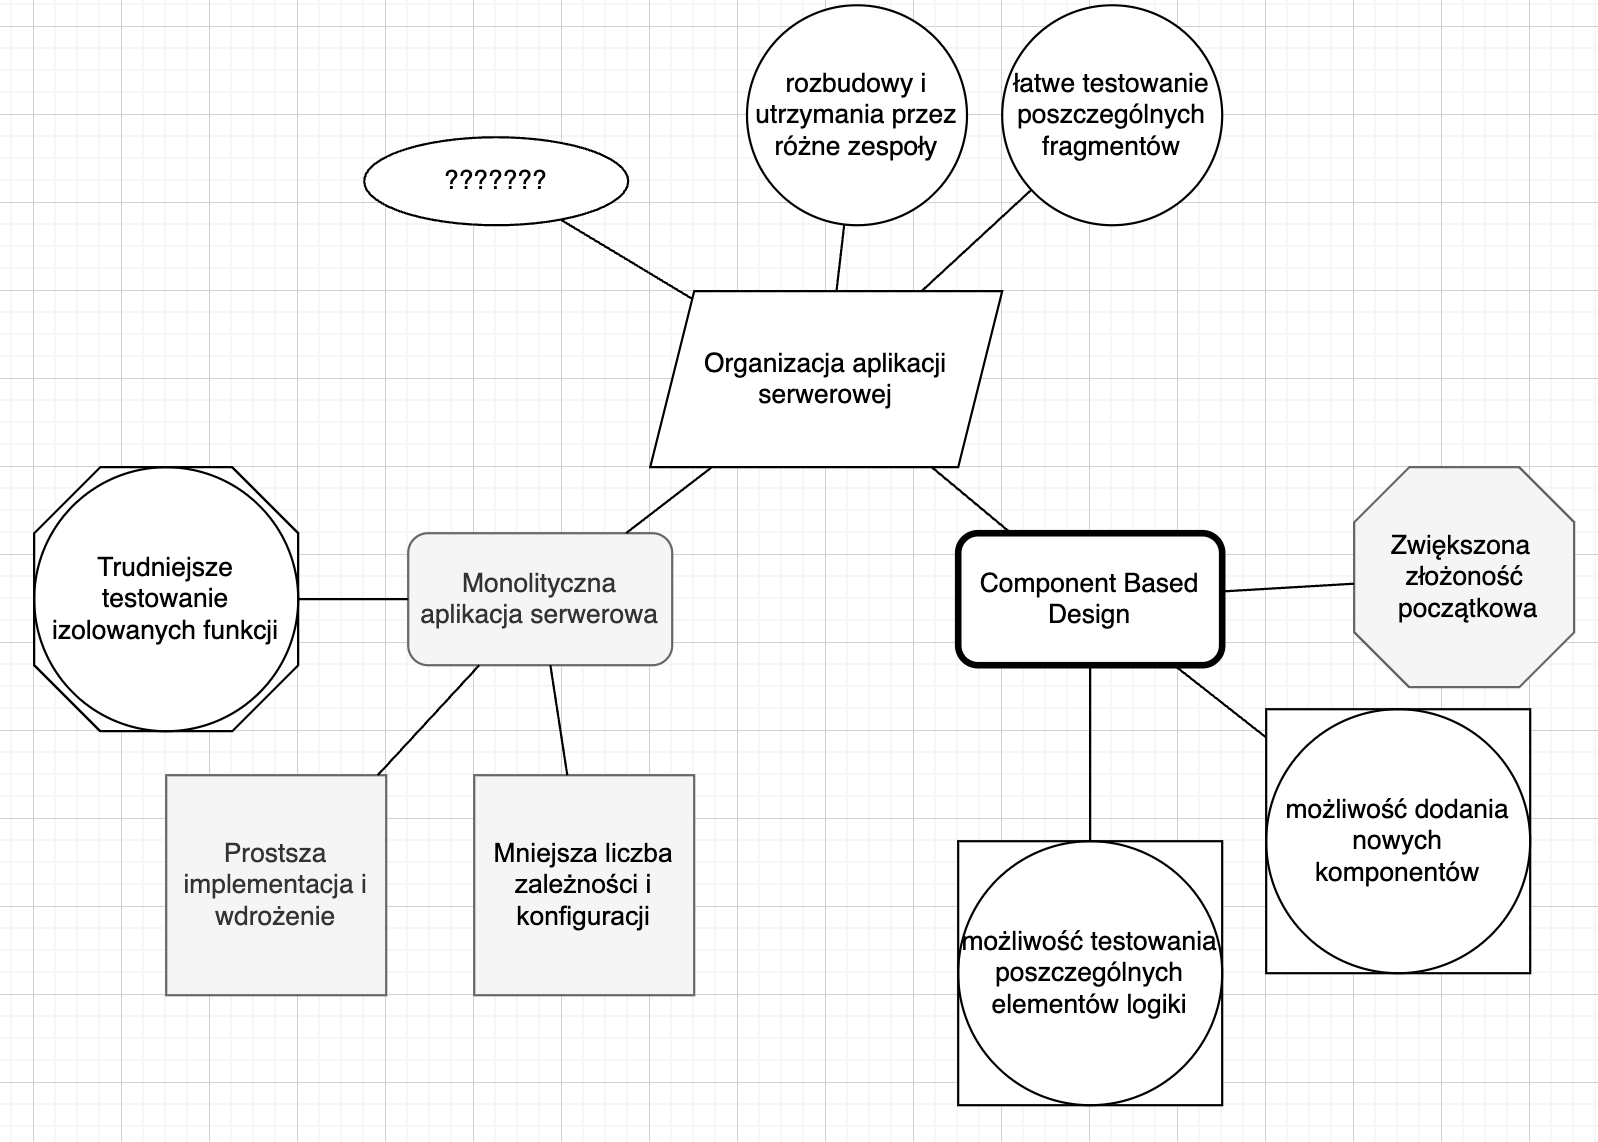
\includegraphics[width=0.8\textwidth]{organizacja_aplikacji_serwerowej.png}
\caption{Diagram podziału na warstwy}
\label{fig:layers}
\end{figure}

\begin{itemize}
\item Warstwa prezentacji: trzy różne aplikacje klienckie — aplikacja webowa, mobilna i aplikacja na urządzenia embedded.
\item Warstwa logiki biznesowej: centralna aplikacja serwerowa (serverApp), w której znajdują się komponenty takie jak UserService, PaymentService, PositionService itd.
\item Warstwa dostępu do danych: komponenty UserRepository, PaymentRepository.
\item Warstwa danych: baza danych Oracle z mechanizmem failover.
\end{itemize}

\textbf{Decyzja:} Rozdzielenie odpowiedzialności na warstwy zwiększa modularność i ułatwia zarządzanie kodem oraz jego testowanie.

\textbf{Alternatywa:} Architektura mikroserwisowa

\textbf{Zalety alternatywy:}
\begin{itemize}
\item Lepsza skalowalność poszczególnych komponentów
\item Możliwość niezależnego wdrażania i rozwijania usług
\item Lepsza odporność na awarie (awaria jednego serwisu $\neq$ awaria całego systemu)
\end{itemize}

\textbf{Wady alternatywy:}
\begin{itemize}
\item Większa złożoność wdrożeniowa (DevOps, CI/CD, monitoring)
\item Konieczność rozwiązywania problemów związanych z komunikacją między serwisami
\item Trudniejsze debugowanie i testowanie end-to-end
\end{itemize}

\subsection{Modularność i komponenty (Component-based Design)}
\begin{figure}[h]
\centering
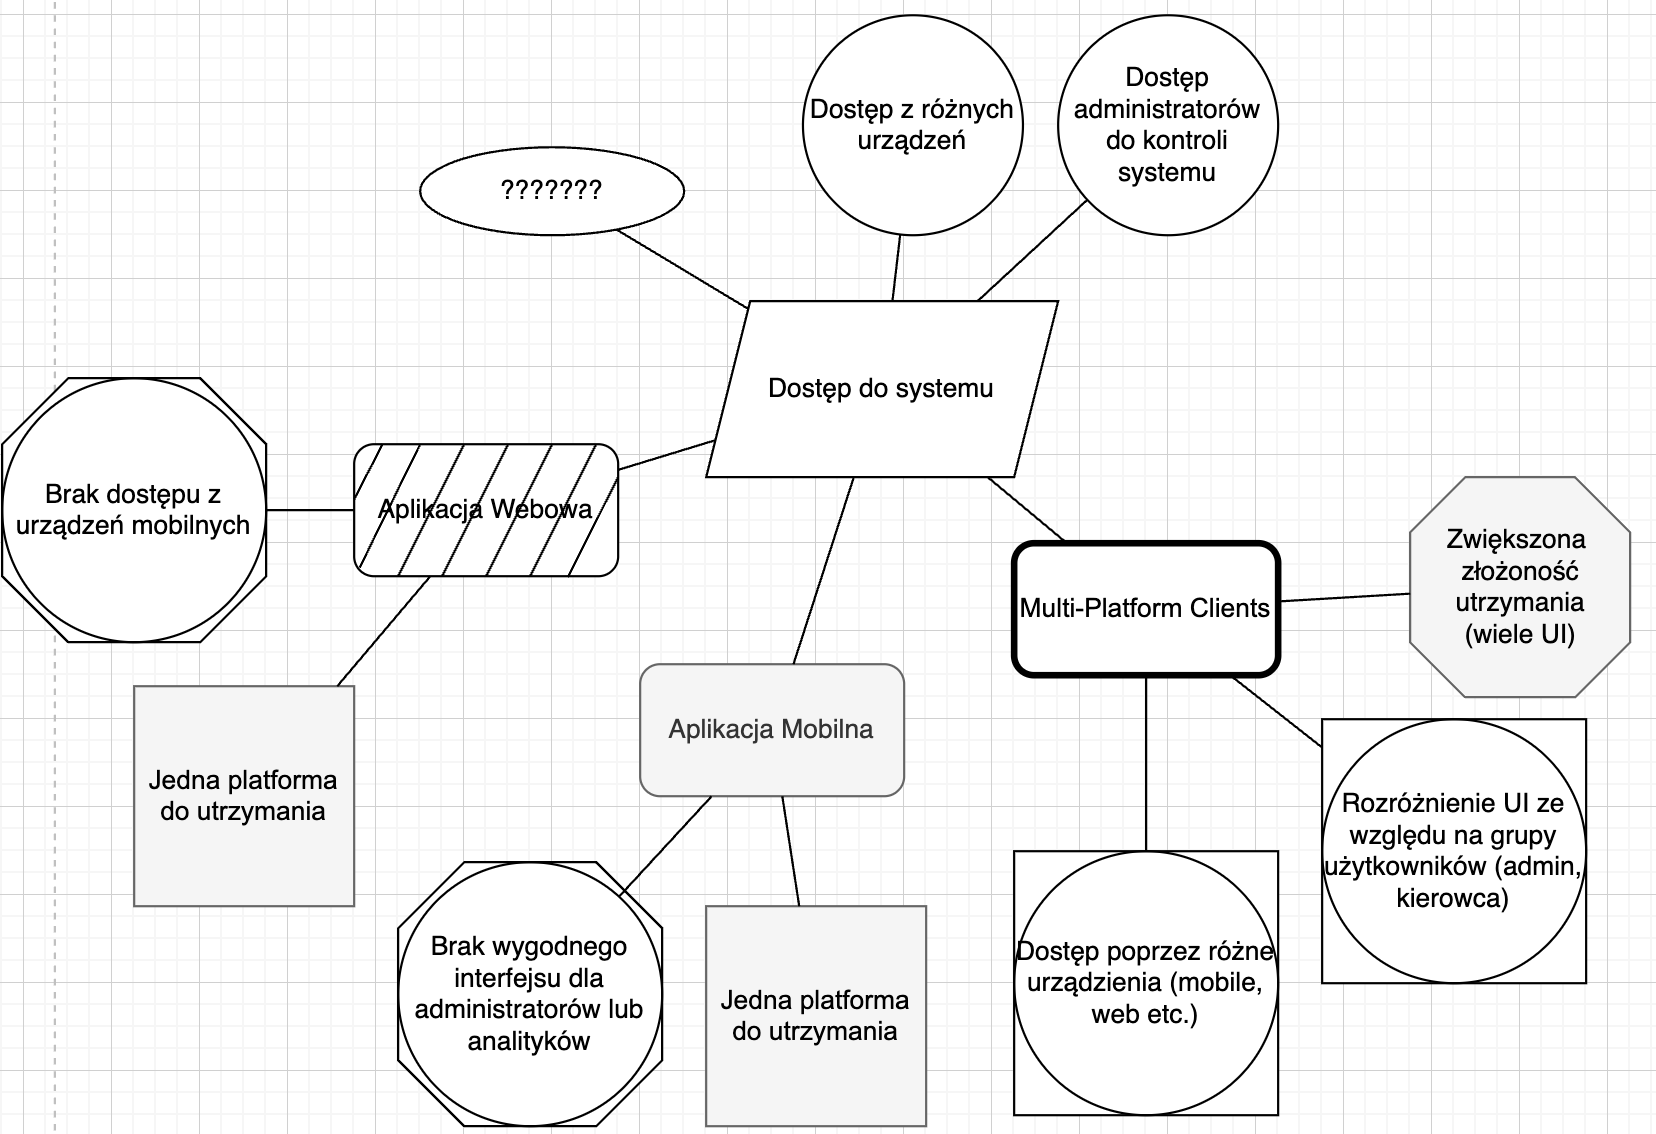
\includegraphics[width=0.8\textwidth]{dostep_do_systemu.png}
\caption{Diagram komponentów}
\label{fig:components}
\end{figure}

\begin{itemize}
\item Serwerowa aplikacja została podzielona na komponenty pełniące konkretne role (SigninController, TollController, MainComponent, itd.).
\item Każdy komponent ma jasno zdefiniowaną odpowiedzialność, zgodnie z zasadą Single Responsibility Principle.
\end{itemize}

\textbf{Decyzja:} Wprowadzenie komponentów umożliwia łatwe rozszerzanie i testowanie poszczególnych fragmentów systemu.

\textbf{Alternatywa:} Monolityczna aplikacja serwerowa

\textbf{Zalety alternatywy:}
\begin{itemize}
\item Prostsza implementacja i wdrożenie
\item Mniejsza liczba zależności i konfiguracji
\item Mniej złożone środowisko developerskie
\end{itemize}

\textbf{Wady alternatywy:}
\begin{itemize}
\item Trudniejsza skalowalność i refaktoryzacja
\item Każda zmiana wymaga redeploy całej aplikacji
\item Trudniejsze testowanie izolowanych funkcji
\end{itemize}

\subsection{Wielokanałowy dostęp (Multi-Platform Clients)}
\begin{figure}[h]
\centering
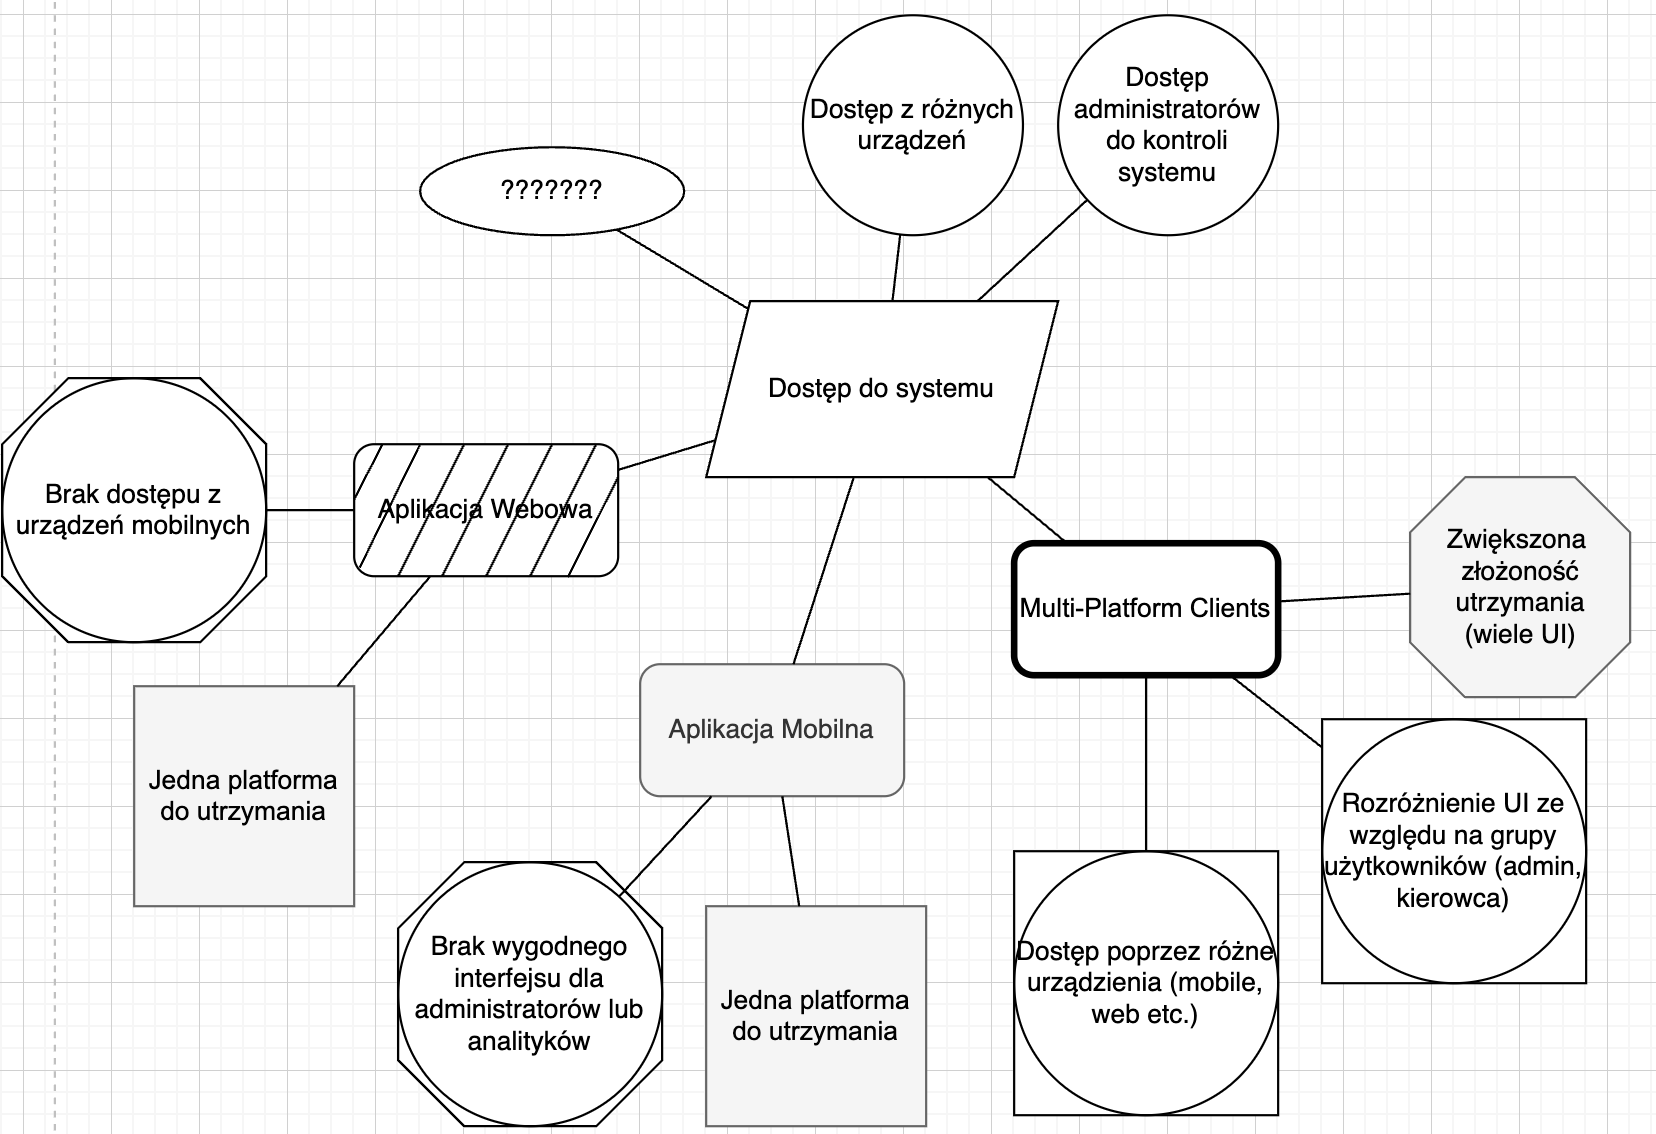
\includegraphics[width=0.8\textwidth]{dostep_do_systemu.png}
\caption{Diagram wielokanałowego dostępu}
\label{fig:multichannel}
\end{figure}

\begin{itemize}
\item Użytkownicy mogą korzystać z systemu za pomocą aplikacji mobilnej, webowej lub urządzeń embedded.
\end{itemize}

\textbf{Decyzja:} Umożliwienie różnym grupom użytkowników (np. administratorzy vs kierowcy) dostępu do funkcji systemu w najbardziej dogodny sposób.

\textbf{Alternatywa:} Tylko aplikacja mobilna (np. PWA lub natywna)

\textbf{Zalety alternatywy:}
\begin{itemize}
\item Uproszczony interfejs użytkownika
\item Jedna platforma do utrzymania
\item Lepsze dopasowanie do kontekstu użytkownika (kierowcy)
\end{itemize}

\textbf{Wady alternatywy:}
\begin{itemize}
\item Brak wygodnego interfejsu dla administratorów lub analityków
\item Mniejsza elastyczność użytkowania
\item Trudności z dostępem do systemu z urządzeń stacjonarnych
\end{itemize}

\subsection{Rozdzielenie ról i uprawnień}
\begin{figure}[h]
\centering
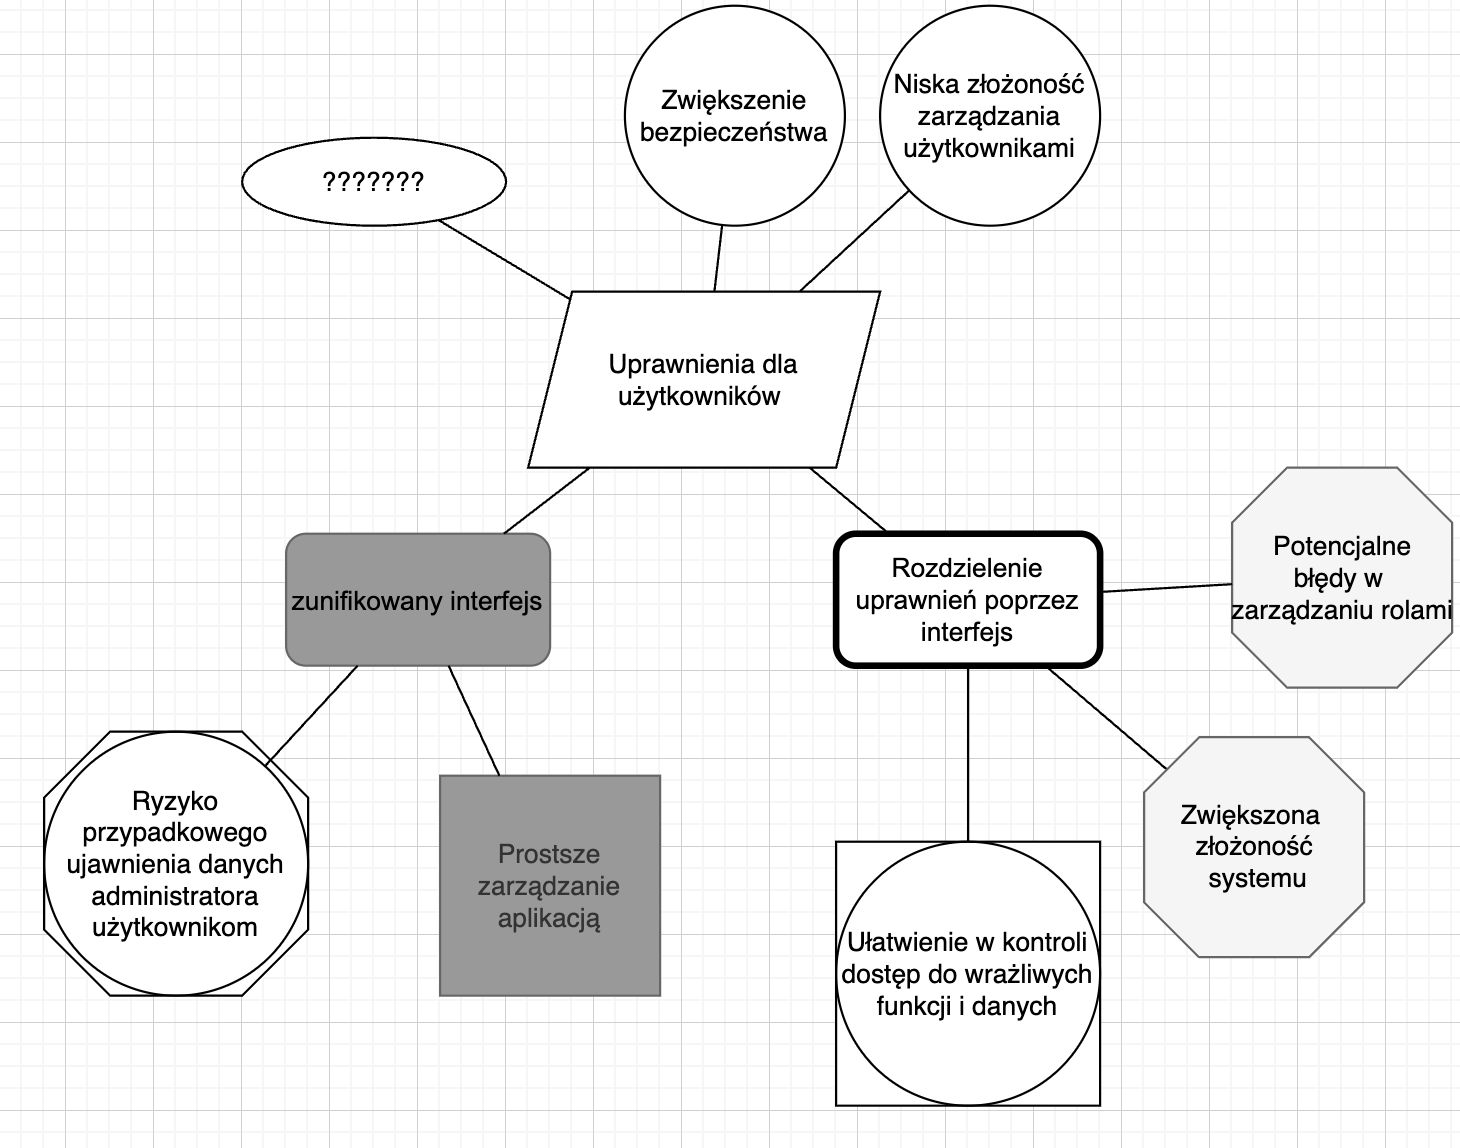
\includegraphics[width=0.8\textwidth]{uprawnienia_dla_uzytkownikow.png}
\caption{Diagram ról i uprawnień}
\label{fig:roles}
\end{figure}

\begin{itemize}
\item Administrator ma dostęp tylko przez aplikację webową.
\item Kierowca może korzystać z trzech różnych interfejsów — w zależności od potrzeb.
\end{itemize}

\textbf{Decyzja:} Jasny podział ról zwiększa bezpieczeństwo i ergonomię systemu.

\textbf{Alternatywa:} Jeden zunifikowany interfejs z uprawnieniami na poziomie konta

\textbf{Zalety alternatywy:}
\begin{itemize}
\item Mniejsze zróżnicowanie UI
\item Mniej kodu i testów związanych z różnymi platformami
\end{itemize}

\textbf{Wady alternatywy:}
\begin{itemize}
\item Mniejsza przejrzystość
\item Możliwość przypadkowego ujawnienia funkcji nieprzeznaczonych dla danego typu użytkownika
\end{itemize}

\subsection{Integracja z zewnętrznymi systemami}
\begin{figure}[h]
\centering
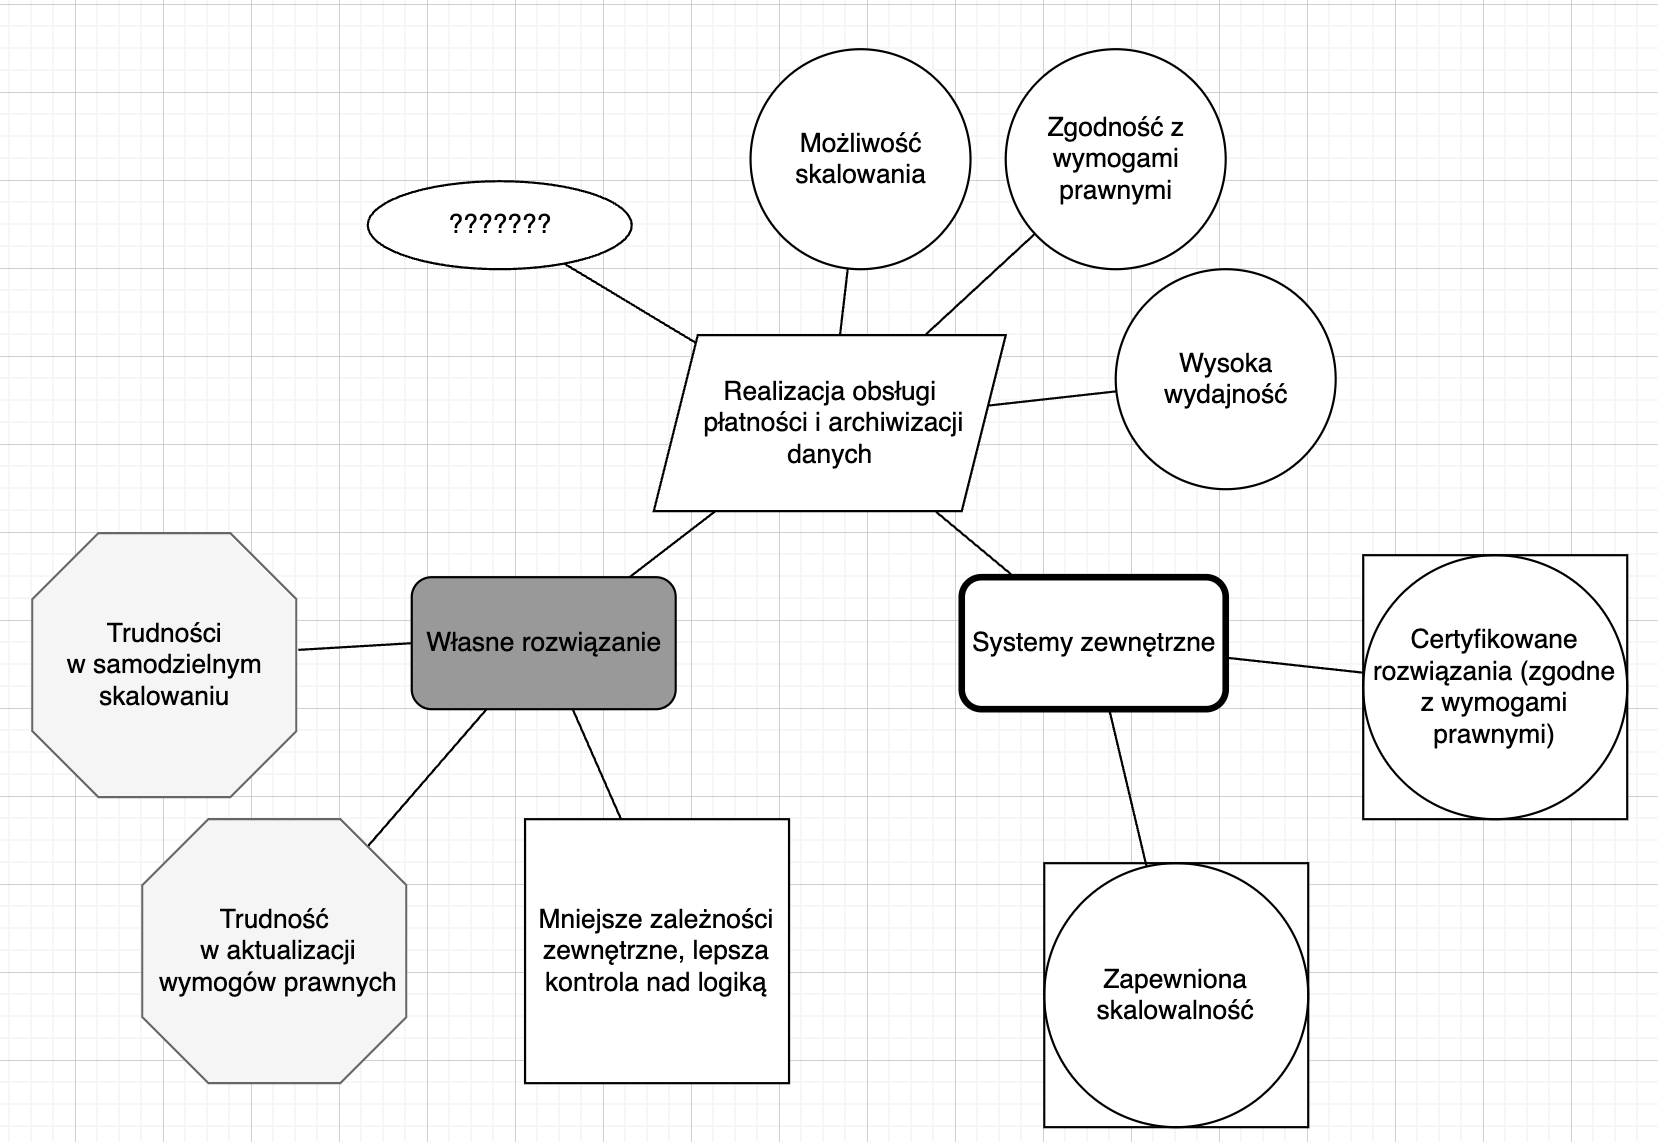
\includegraphics[width=0.8\textwidth]{realizacja_obslugi_platnosci_i_archiwizacji_danych.png}
\caption{Diagram integracji z systemami zewnętrznymi}
\label{fig:integration}
\end{figure}

\begin{itemize}
\item System płatności (systemPlatnosci) oraz system archiwizacji danych (archiwum) są zewnętrznymi systemami zintegrowanymi z systemem e-Toll.
\end{itemize}

\textbf{Decyzja:} Wydzielenie tych odpowiedzialności do zewnętrznych systemów pozwala na lepsze skalowanie oraz wykorzystanie istniejących rozwiązań.

\textbf{Alternatywa:} Wszystko w ramach jednej aplikacji (np. własny moduł płatności i archiwizacji)

\textbf{Zalety alternatywy:}
\begin{itemize}
\item Większa kontrola nad logiką
\item Mniejsze zależności zewnętrzne
\end{itemize}

\textbf{Wady alternatywy:}
\begin{itemize}
\item Większe ryzyko błędów w obszarach regulowanych prawnie (np. płatności)
\item Większe koszty utrzymania i certyfikacji
\item Brak skalowalności i elastyczności
\end{itemize}

\subsection{Wysoka dostępność i odporność na awarie}
\begin{figure}[h]
\centering
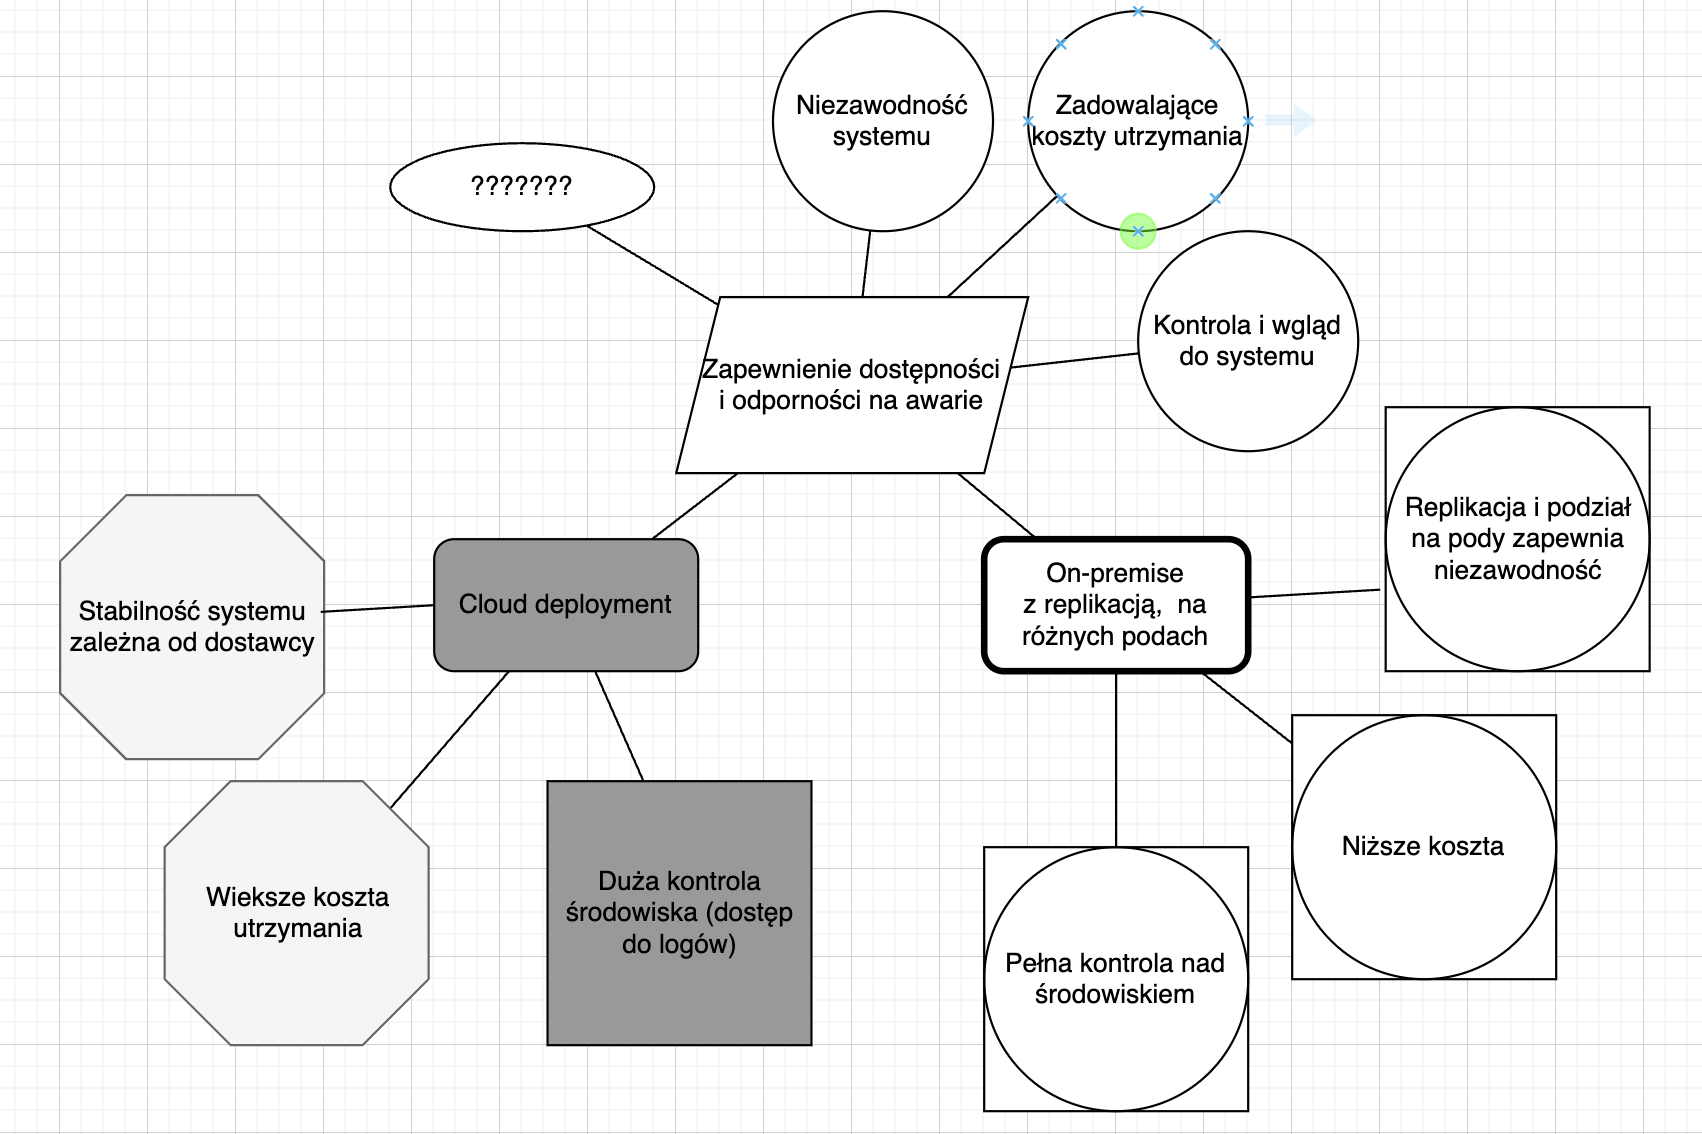
\includegraphics[width=0.8\textwidth]{zapewnienie_dosepnosci_i_odpornosci_na_awarie.png}
\caption{Diagram wysokiej dostępności}
\label{fig:high-availability}
\end{figure}

\begin{itemize}
\item Baza danych jest replikowana (primary–secondary).
\item Oddzielne deployment node'y dla różnych typów urządzeń oraz dla aplikacji serwerowej i bazy danych.
\item Failover serwera bazy danych — Oracle - Secondary.
\end{itemize}

\textbf{Decyzja:} Architektura uwzględnia mechanizmy zapewniające ciągłość działania systemu nawet w przypadku awarii.

\textbf{Alternatywa:} Deployment w chmurze

\textbf{Zalety alternatywy:}
\begin{itemize}
\item Duża skalowalność
\item Bezpieczeństwo i redundancja
\end{itemize}

\textbf{Wady alternatywy:}
\begin{itemize}
\item Wyższe koszty
\item Przetwarzanie danych przez inne podmioty
\end{itemize}

\subsection{Wybór technologii wdrożeniowych}
\begin{figure}[h]
\centering
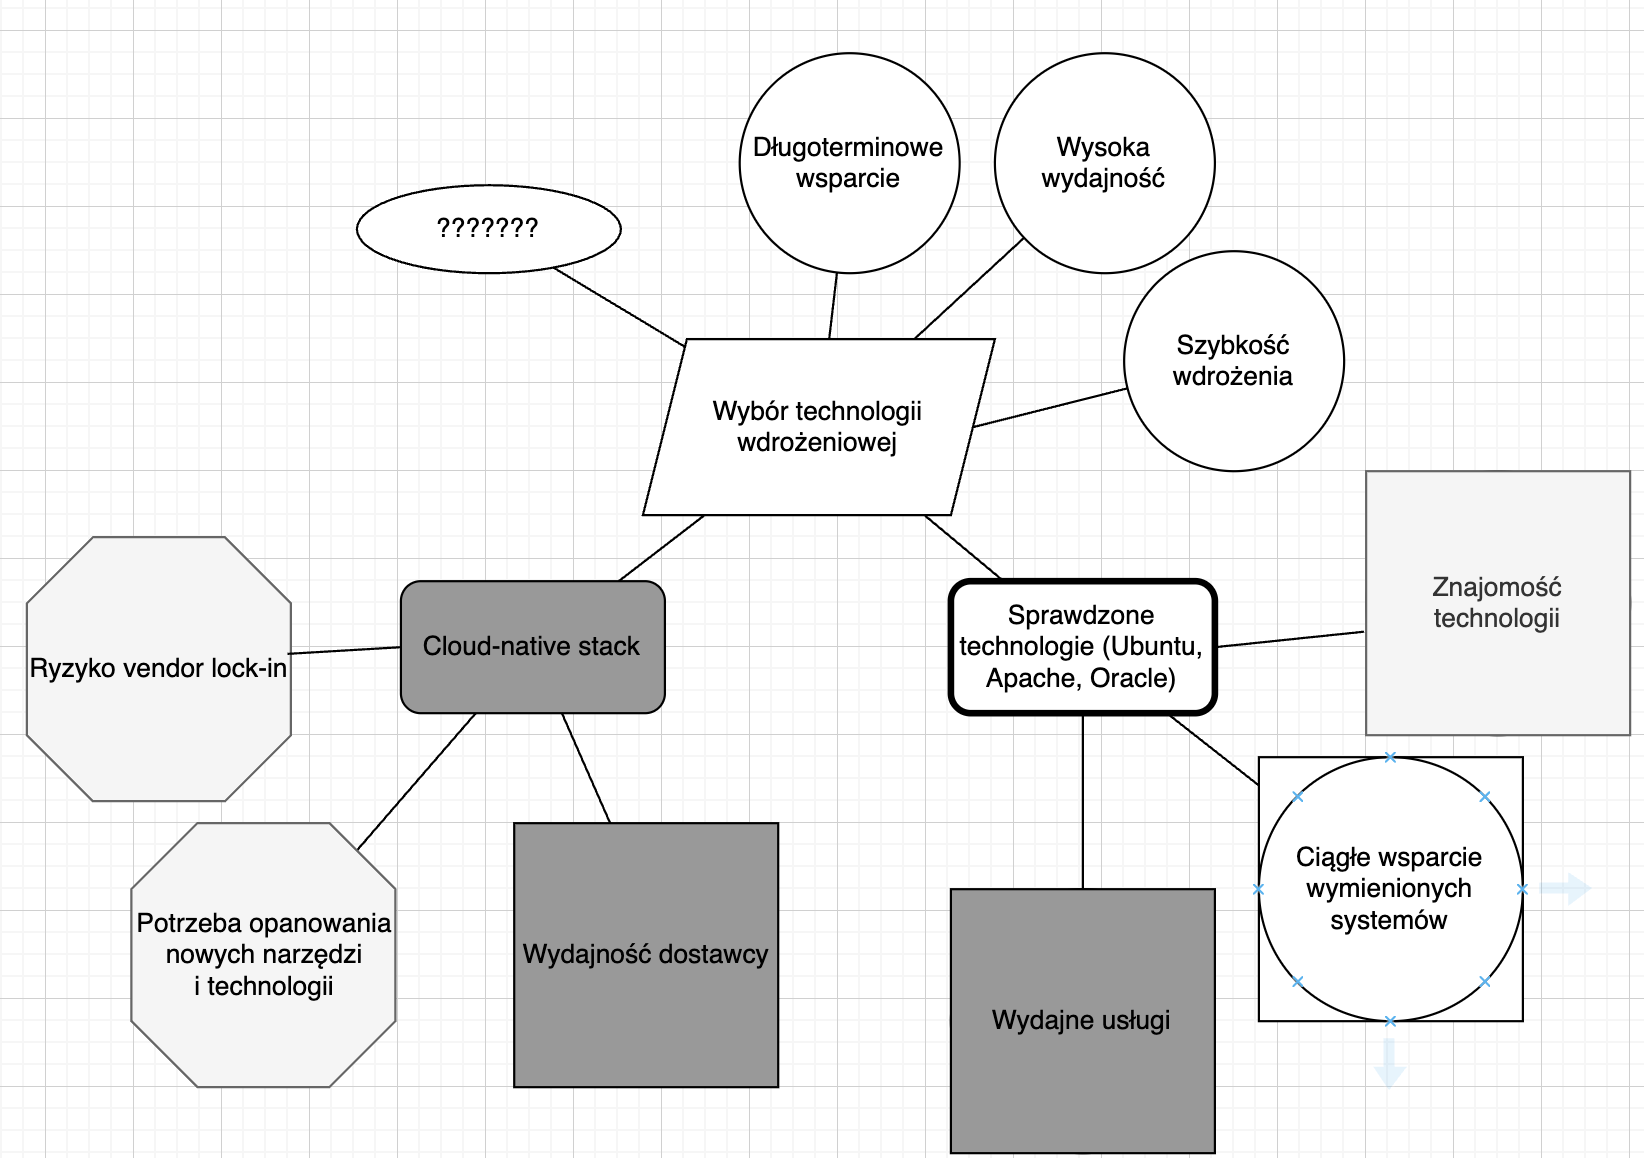
\includegraphics[width=0.8\textwidth]{wybor_technologii_wdrozeniowej.png}
\caption{Diagram technologii wdrożeniowych}
\label{fig:deployment-tech}
\end{figure}

\begin{itemize}
\item System hostowany na serwerach z Ubuntu 24.04 LTS.
\item Serwer aplikacji oparty o Apache Tomcat 8.x.
\item Baza danych Oracle 12c.
\end{itemize}

\textbf{Decyzja:} Użycie sprawdzonych technologii o długoterminowym wsparciu i wysokiej wydajności.

\textbf{Alternatywa:} Cloud-native stack – np. AWS/GCP

\textbf{Zalety alternatywy:}
\begin{itemize}
\item Automatyczne skalowanie, monitoring, CI/CD
\item Niższe koszty utrzymania fizycznej infrastruktury
\item Łatwiejsze zarządzanie kontenerami i usługami
\end{itemize}

\textbf{Wady alternatywy:}
\begin{itemize}
\item Uzależnienie od chmury (vendor lock-in)
\item Potrzeba opanowania nowych technologii
\item Potencjalne wyższe koszty początkowe
\end{itemize}

\end{document}
